\documentclass[10pt]{article}
\usepackage{multicol}
\usepackage{authblk}
\usepackage{mathptmx}
\usepackage{graphicx}
\setlength{\columnsep}{5mm}
\usepackage{blindtext}
\usepackage{geometry}
\usepackage{url}
\usepackage{listings}
\usepackage{xcolor}
\usepackage{float}
\usepackage{longtable}
\usepackage{cite}


\definecolor{codegreen}{rgb}{0,0.6,0}
\definecolor{codegray}{rgb}{0.5,0.5,0.5}
\definecolor{codepurple}{rgb}{0.58,0,0.82}
\definecolor{backcolour}{rgb}{0.95,0.95,0.92}

\lstdefinestyle{mystyle}{
    backgroundcolor=\color{backcolour},   
    commentstyle=\color{codegreen},
    keywordstyle=\color{magenta},
    numberstyle=\tiny\color{codegray},
    stringstyle=\color{codepurple},
    basicstyle=\small,
    columns=flexible,
    breakatwhitespace=false,         
    breaklines=true,                 
    captionpos=b,                    
    keepspaces=true,                 
    numbers=left,                    
    numbersep=2pt,                  
    showspaces=false,                
    showstringspaces=false,
    showtabs=false,                  
    tabsize=2
}

\lstset{style=mystyle}

\geometry{
  a4paper,
  left = 20mm,
  top = 2mm,
  right = 20mm
}

\title{\textbf{Parallel dragonfly algorithm} %
  \\[2ex] \large High Performance Computing for Data Science course 2024/2025}

\author[1]{Mattia Santaniello}
\author[2]{Alessio Zeni}
\affil{University of Trento}

\begin{document}

\maketitle

\begin{multicols}{2}[
  \fontsize{9}{9}
  \section*{Abstract}
  \textbf{Dragonfly algorithm is a new kind of approach used to solve optimization problems through the emulation of dragonflies movements, but it lacks scalability. In this paper the authors try to set up an approach based on parallelization thanks to the use of API for high performance computing like MPI and OpenMP, then there will be a comparison of execution times between presented implementation and the classic approach based on serial programming, in order to see if parallelization could lead to a performance improvement and possible future extensions.}\newline]

\section{Introduction}

Recent years have seen the raise and evolution of swarm intelligent algorithms, based on meta-heuristic approach where single individuals of a complex population follow an exploration-exploitation methodology to find the best solution in their local search space;
each member of the group work independently from the others, leading to a subdivision of the labour which decrease the overall amount of execution time, working as decentralized and parallel units; but also, due to the fact that they mimic the behaviour of biological life forms, it is possible then that they could generate random patterns through the interaction with each other. 
The dragonfly algorithm has been proposed for the first time in 2016, and its purpose is to simulate the behaviour of a dragonfly population according to the principles of swarm intelligent algorihms seen previously.
It has gained more and more popularity: it is in estimated that during 2019 more than 300 scientific papers cited the algorithm \cite{DASurvey}, due to the fact that it has demonstrated some characteristics similar to other algoritms of the same kind, however in contrast with other swarm intelligent algorithms however it present less probability to be trapped into a local optima \cite{DAReview}.
This paper aims to define a new approach based on popular parallel APIs, and also trying to understand if parallelization could lead to a significant speed up in performances that can be considered by future researches on this algorithm 

\subsection*{How the algorithm works}
The execution begins with the initialization of some arrays which are the position $P$ of all dragonfiles and the `step` vector $\Delta P$ representing the velocities of each single individual,the position of source foods $F$ and the position of enemies $E$;
then the algorithm executes an iteration loop where, for each dragonfly, we calculate some coefficient that will be used to update the internal state of the program.
This procedure is simulated through the observation of repetitive patterns observed in the behaviour of dragonflies, which are:



\begin{itemize}
  \item Alignment of their velocity with other members of the same group, given by the formula  $A_i = \frac{\sum^M_{j=1}V_j}{M}$, where $V_j$ is the velocity of the j-th neighbour

  \item Separation of single members in order to avoid collision, and it is retrieved by the equation  $S_i = - \sum^M_{j=1}{P - P_j}$, where $P_j$ is the position of the j-th neighbour and $P$ the current individual position.
    
  \item Cohesion towards the center of the group, given by $C_i = \frac{\sum^M_{j=1}P_j}{M} - P$ 
  \item Attraction to a common source food, expressed by the formula $ F_i = F^+ - P$, where $F^+$ is the position of the current prey and $P$ is the position of the current dragonfly
  \item Distraction of enemies, represented by the equation $ E_i = E^- + P$ where $E^-$ is the position of the current enemy 
\end{itemize}

\noindent Once all the parameters have been calculated we can now update the current step vector of each dragonfly using the following equation: $$\Delta P^{t+1}_{i} = (sS_i + aA_i + fF_i + cC_i) + \omega\Delta P^t_i$$ where $s,a,f,c$ are respectevly the separation weight, the alignment weight, the attraction weight, the cohesion weight and $\omega$ is the inertia weight, all of them are randomly chosen in the interval $[0,1]$. When all step vectors have been updated we can now set the new position of the dragonflies using this equation, which takes the new step vector as an input: $$P^{t+1}_{i} = P_i^t + \Delta P_{i}^{t+1}$$However if there is a dragonfly which does not have any neighbour then we assume that the overall population moves in a random way: the most common method to do that is to use a random walk function. The previous formula then must be modified into this one here: $$P^{t+1}_i = P_i^t + Levy(d)$$ where $d$ is the dimension of the position vector, and $Levy(d)$ is the Levy flight function, which is calculated in this way: $$Levy(d) = 0.01\times\frac{r_1 \times \sigma}{|r_2|^{\frac{1}{\beta}}}$$ where $r1$ and $r2$ are two random numbers uniformally distributed in the interval $[0,1]$, and $\sigma$ is a vector calculated using the following formula: $$\sigma = \frac{sin(\frac{\beta\pi}{2})\times\Gamma(1+\beta)}{\Gamma(\frac{\beta+1}{2})\times \beta \times 2^{(\beta-1)/2}}$$ where $\Gamma(x)$ is the gamma function \cite{WikiGamma}, and $\beta$ is a constant.Another valid approach is to apply, instead of Levy flight, the brownian motion model, used especially in gas and particle analysis: this seems to return better performances \cite{BDragonfly}. 




\section{General approach}

Now that we have seen the overall procedure it is possible to write a naive implementation of the algorithm in order to 
have a base for further developments. An example of the implementation can be observed in the following code snippet:


\begin{lstlisting}[language=C,caption={first implementation of the dragonfly algorithm}]
void dragonfly_algorithm(Dragonfly *d, 
                        float *average_speed,
                        float *cumulated_pos, 
                        float *food, 
                        float *enemy,
                        unsigned int N, 
                        unsigned int random_seed) {

  unsigned int dimensions = d->dim;
  float S;
  float A;
  float C;
  float F;
  float E;
  float levy;

  float *cur_pos;
  float *cur_speed;

  for (unsigned int j = 0; j < d->N; j++) {
    unsigned random = random_seed + j;
    cur_pos = d->positions + j * dimensions;
    cur_speed = d->speeds + j * dimensions;

    // compute speed = sSi + aAi + cCi + fFi + eEi + w

   for (unsigned int i = 0; i < dimensions; i++) {
      S = ((cumulated_pos[i] - cur_pos[i]) / (float)N);
      A = average_speed[i];
      C = (cumulated_pos[i] / (float)N) - cur_pos[i];
      F = food[i] - cur_pos[i];
      E = enemy[i] + cur_pos[i];
      levy = RAND_FLOAT(1.0, &random);

      cur_speed[i] *= d->w.w;
      cur_speed[i] += d->w.s * S;
      cur_speed[i] += d->w.a * A;
      cur_speed[i] += d->w.c * C;
      cur_speed[i] += d->w.f * F;
      cur_speed[i] += d->w.e * E;
      cur_speed[i] += levy;

      cur_pos[i] += cur_speed[i];
    }
  }
}
\end{lstlisting}

\noindent After the initialization of velocities and positions of agents,
which will be represented by two separated matricies with the same dimension equal to the number of members of our
population times the dimension of our problem, the algorithm starts to execute a for loop 
with a fixed amount of iteration stored in the variable $d\rightarrow N$,  retrieve
the position and the velocity of the current dragonfly, represented by pointers
\textit{cur\_pos} and \textit{cur\_speed},
and the cumulated coordinates of its neighbours. 
The execution then proceed with the following steps:

\begin{itemize}
  \item retrieve current speed and position of the j-th dragonfly
  \item compute separation, alignment, cohesion, food attraction and enemy distraction vectors,
  stored into local variables named with their abrreviations
  \item calculate product between weigths and and the single coordinates of the velocity array
  \item update speed and position the dragonfly considering also brownian motion
\end{itemize}

\noindent Notice how the computation
of velocities and speed coordinates is compacted into the same \textbf{for} loop;
this allows to reduce time execution, because the overall calculation is made locally
all in the same place, leaving out the necessity of using auxiliary arrays for the coefficients.
The reason why we divide the separation coefficient for the number of neighbours 
will be explained later in this paper

\subsection*{chunks}

As anticipated earlier dragonfly algorithm, as many other swarm optimization solutions,
has a good chance to be stuck into a local minima, without the possibility to find better
candidates. We can avoid this and improve this approach introducing groupments of dragonflies into chunks, 
calculating local minima of different areas and compare them in order
to get as close as possible to the global solution.  

\begin{figure}[H]
  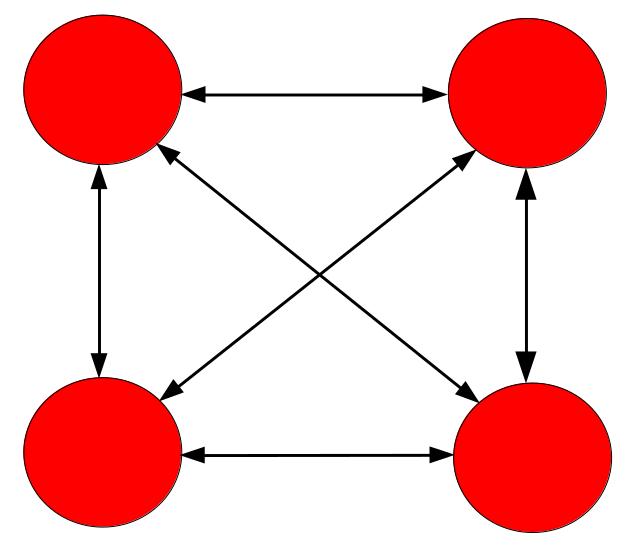
\includegraphics[scale=0.3]{img/chunks.png}
  \centering
  \caption{illustration of communication between chunks}
\end{figure}

\noindent The implementation of this process is quite simple: each chunk will contain a subset
of components of the global population that will specialize to compute the point with the best local
fitness for both enemies and food of that specific region, then the local status will be communicated
to all other chunks, updating in this way the global status of the program thanks to the update of positions,
and the local configuration of each region; the algorithm ends displaying the best fitness found
during the execution.


\section{Critical analysis of the coefficients}
From this implementation we discovered some critical points that should be improved:
\begin{itemize}
  \item In the original paper\cite{Original} and in the algorithm often uses the therm neighbours without giving a precise definition.
  Assuming a general distance metric (eg Euclidean Distance), could be an option, but later in the paper it describes how the alghorithm runs in linear time with respect to the number of dragonflies and the iteration count.
  This would be false in case of euclidean distance, because in order to define for each butterfly the neighbours, we should calculate the distance between each pair of dragonflies, which would lead to a time complexity of $O(N^2)$.
  Maybe using some complex geospatial algorithms it could be possible to archive that, but we doubt this was the original intention of the authors.
  Later in the paper also another crithical problem in respect to other algorithm was the premature convergence. So we decided to divide the population in chunks, and progressively merge chunks until we will remain with only one.
  So in this way we addressed both problems.
  \item In order to be a solid algorithm it must be garanteed that does not exist some values that would make the solution diverge.
  As a first approach we introduced a max\_speed\ parameter that would change over time and would assure stability. 
  But given that in the original paper it was not described we omitted from later implementations.
  This lead to instabilities from the enemy coefficient (if bigger than 0.5), but mainly from the separation coefficient.
  This is a problem, because we could be see the coefficient as n times the distance between the dragonfly and the average position of the population. For example if the distance is 0.001, 
  but there are 1000 dragonflies in the neighbourhood, then the coefficient would be 1, at the very next iteration the dragonflies would have a distance of 1 from the center and so on, causing an exponential growth.
  In order to fix this we modify the separation formula as: $S_i = - \frac{\sum^M_{j=1}{P - P_j}}{M}$.

  \item  The enemy coefficient does not represent what the author describes. The sum of vectors does not necessarily point outwards in respect to the enemy (eg with aligned pos vectors). 
  We assumed a typo, but even the difference of the vectors would not be enough, because if the enemy is too close to the dragonfly, the difference would get smaller and not bigger.
  A possible solution would be to normalize the difference vector with the inverse of the vector length, but the formulation would have been to different from the original one. So we decided to keep the original formulation and see if it actualy would do something.
\end{itemize}


\section{Parallelization with MPI}

OpenMPI is a library that enables code execution on multiple cores, wheter they belong
to the same CPU or not; it can be useful in case of performace improvement of those algorihms
that require to solve complex tasks, just like the dragonfly algorithm: in fact this library can be easily 
adapted to the illustrated implementation in order to boost performance.

\subsection*{MPI on chunks}
As we said earlier chunks are independent from each otherm but usually they need to comunicate
with their neighbours in order to keep updated the global status of the program execution. 
It is possible to run chunks groups simoultaneously, using MPI builtin function to connect 
the processes.  The instructions computed by each process are available in a custom function
called \textit{dragonfly-compute}; after calculating the ID of the initial and final chunks
and initializing message structures using the \textbf{offsetof} macro
the function will execute the update loop that calculates the new velocities and positions 
of the dragonfly for each chunk associated. To do this we first need to update the current
location of enemies and food present in the chunk using the function \textbf{computation\_status\_merge},
using the position of food and enemies of other chunks retrieved by the function \textbf{message\_broadcast};
finally the process will proceed to update current position and velocities of dragonfiles using 
the function \textbf{dragonfly\_compute\_step} illustrated earlier

\subsection*{MPI and parameters}
Since MPI has been useful in the parallelization of the chunks then it can also become useful in
the training of parameters.

\section{OpenMP implementation}

OpenMP is a low level API that allows us to execute a sequence of instructions on different threads belonging
to the same CPU core, improving in this way the performances of our implementation. This feature can be used to 
speed up the execution of some slow functions, in our case these will be dragonfly-compute-step and message-accumulate

\subsection*{General use}

First of all it is necessary to understand how OpenMP should be inserted in the code: first of all we have to use 
a compiler that supports this technology, in our case we have gcc, which allows OpenMP execution thanks to the flag -fopenmp.
Second we need to include a pragma directive in our code, which will wrap the set of instructions that we are interested to execute
in parallel. Since the implemented results will perform loops mainly then it is fundamental to calculate the work balance between the number of iterations, if the main
body is a loop,
and the number of threads available. Each thread has to define the starting and the end point of the loop that has to execute,
calculating the starting index as $rank*ratio$ and the end one as $ratio*(rank+1)$, where $rank$ is the ID of the thread

\subsection*{dragonfly-compute-step}

One of the two functions that we are interested to execute using OpenMP is \textit{dragonfly-compute-step}:
if we take a look on the serial version we notice that each computation step is independent
from other iterations. This means that the execution flow can be split in many subtasks assigned
to threads. The following code snippet illustrate how all the procedure has been implemented

\begin{lstlisting}[language=C,caption={parallelized dragonfly-compute-step}]
void dragonfly_compute_step(Dragonfly *d, 
                            float *average_speed,
                            float *cumulated_pos, 
                            float *food, 
                            float *enemy, 
                            unsigned int N, 
                            unsigned int NR_THREADS) {

  unsigned int base_random = rand_r(&d->seed);
  unsigned int rest = d->N % NR_THREADS;
  unsigned int ratio = d->N / NR_THREADS;

  ...

  #pragma omp parallel num_threads(NR_THREADS)
    {
      
      unsigned int rank = omp_get_thread_num();
      //printf("rank=%d\n", rank);
      unsigned int base = ratio * rank;
      unsigned int limit = ratio * (rank + 1);
      inner_dragonfly_step(d, average_speed, 
                          cumulated_pos, food, 
                          enemy, N,
                          base, limit, base_random);
    }
  
  ...

  if (rest != 0) {
      unsigned int r_base = ratio * NR_THREADS;
      unsigned int r_end = d->N;

      inner_dragonfly_step(d, average_speed, 
                           cumulated_pos, 
                           food, enemy, N,
                           r_base, r_end, base_random);
    }
  }

  weights_step(&d->w);
  
  }

\end{lstlisting}


\noindent After we got all basic informations the \textit{inner\_dragonfly\_step}
function can be executed, wrapping it into the \textbf{pragma} directive that we have seen earlier: in this way each thread will 
perform the necessary operations only on a specific portion of the overall positions and speeds arrays.
If the number of threads does not divide perfectly the size of the arrays then we compute the rest
returned from the ratio calculation and the remaining cells will be processed using the serial approach.

\subsection*{computation\_accumulate}

The \textit{computation\_accumulate}  must compute
the cumulated positions and speeds of the chunk and find the best food and enemy positions.
The implementation of a parallelized approach in this case  is more complicated to achieve, 
because threads should read and write on the same memeory areas which could be 
difficult to execute independently from each other. This time it is necessary to define
local buffers for each thread, so they can store temporary results without the risk of using
overlapping memeory locations. 
\begin{figure}[H]
  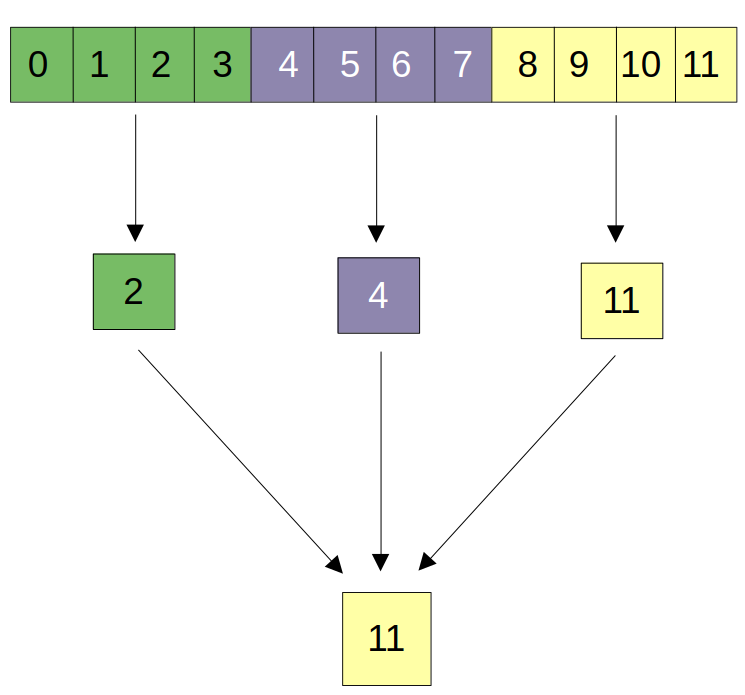
\includegraphics[scale=0.2]{img/reduce-example.png}
  \centering
  \caption{Illustration of the reduce process performed by the computation\_accumulate function}
\end{figure}
\noindent The parallel section provides that each thread must compute the local
cumulated sums of velocities and positions, then they must select the position with the best fitness value
in order to find the best local position of food and enemies. Once the local execution is completed
it will update the global status of the chunk using a critical section, with one thread that can execute that
specific portion of the program

\section{Final execution and results}
Now that we have described all the procedure it is time to illustrate how 
the algorithm has been executed. This job has been performed by the
High Performance Computing cluster at University of Trento, which 
use a particular technology called PBS to handle multiple tasks at the same
time: this feature comes useful in our case since, as we will see later, we 
execute multiple istances of the same problem
\subsection*{structure of the execution}

As anticipated we will execute the same problem using multiple instances with different amount of
resources in order to get a complete evaluation of performance. The overall execution use from 1 to 8
threads, and 4 to 1024 cores

\subsection*{performace theory}

After the end of all tasks it is possible to check how much gain in performance we have obtained.
To do this it is necessary to introduce some theoretical concepts that will give us the tools that
will give us a good metric system to evaluate our results.Speedup is defined as the ratio between the the execution times of the serial and parallel
implementations, so the formula will be equal to: $$Speedup = \frac{T_{serial}}{T_{parallel}}$$ 
from this definition it is obvious that the more the speedup is the more the parallel implementation
performs better. There is a particular case where the time execution of the denominator can be defined
as $T_{parallel}=T_{serial}/p$, where \textit{p} is the number of cores: this is called \textit{linear speedup},
and in this situation it perfectly match with the classic speedup coefficient
Efficiency is another important parameter, and it is defined by the ratio of the speedup and the 
number of cores, giving the following formula: $$E = \frac{Speedup}{p}$$
also in this case the efficiency decrease due to the increase of the number of cores. In case
of linear speedup we get that the efficiency is equal to the inverse of $p$
\subsection*{results}
Now it is possible to show results obtained from the cluster,
using the configuration with 4 cores and 1 thread will be considered
equal as the serial time
\newline

\begin{tabular}{| c | c | c | c | c | c | c |}
  \hline
  T/p & 4	 & 8	& 16	& 32	& 64 & 128  \\
  \hline
  1 & 1	& 2,03 & 3,87 & 7,94 & 14,76 & 31,19  \\
  2 & 1,04 & 2,05 & 3,97 & 8,50 & 16,43 & 27,90 \\	
  4 & 1,01 &2,03	& 4,21 &	8,04 &	16,37 &	35,26	\\	
  8 & 1,02  &2,02 &	4,02 &	8,62 &	18,32 &	32,26 \\
  \hline
\end{tabular}
\newline\newline As we can see the speedup tends to 
increase when the number of cores increase, however when
we use more threads it happens that the
speedup start to decrease at a certain point for some
core configuration. As we can see from the plots it 
seems there are threshold at some specific points, depending
on the number of threads used; notice how the inclinations
of the lines in the plot tends to be less and less evident.

\begin{figure}[H]
  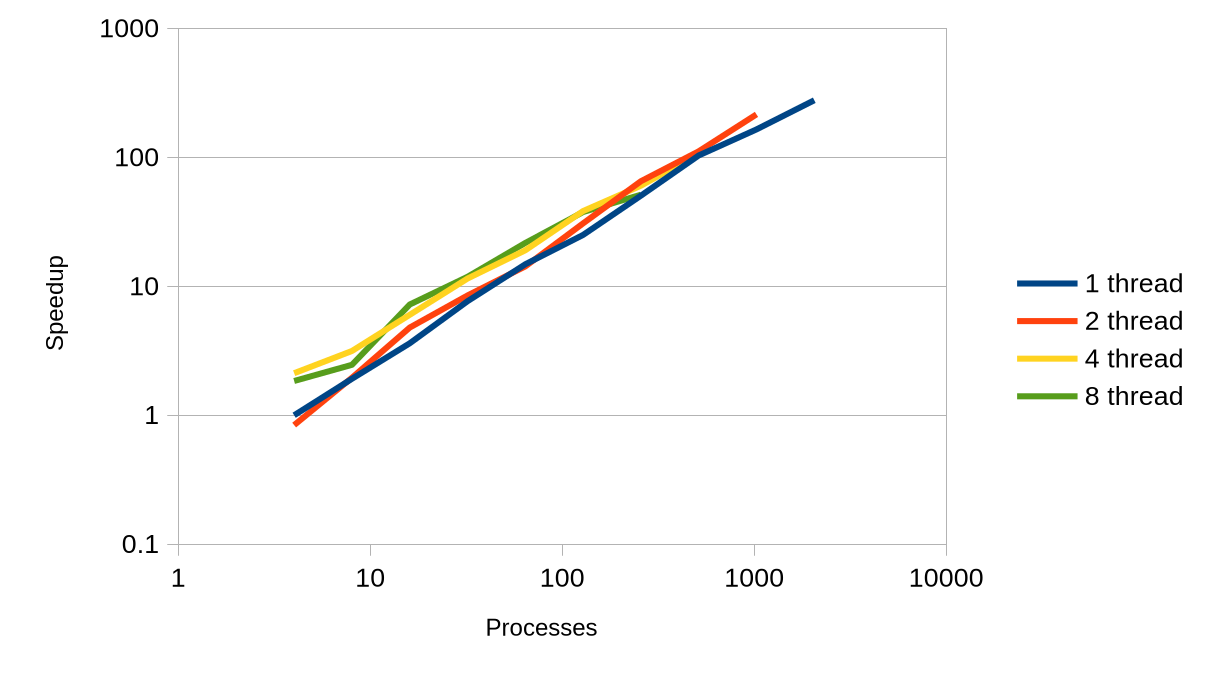
\includegraphics[scale=0.3]{img/speedup.jpg}
  \centering
  \caption{speedup graphic}
\end{figure}

\noindent 
Efficiency tends to present an unpredictable behaviour,
in fact the coefficients grows for some particular setups,
for others instead numbers decrease. If we take a look on
the plot below it shows that there is a high variance in the
datas, with the lines that tends to be more stretched when the
number of threads gets higher
\newline
\newline
\begin{tabular}{| c | c | c | c | c | c | c |}
  \hline
  T/p & 4	 & 8	& 16	& 32	& 64 & 128  \\
  \hline
  1 & 1	& 1,02 & 0,97 & 0,99 & 0,92 & 0,97  \\
  2 & 1,04 & 1,03 & 0,99 & 1,06 & 1,03 & 0,87 \\	
  4 & 1,01	&1,01&	1,05&	1&	1,02&	1,1	\\	
  8 &1,02&	1,01&	1,01&	1,08&	1,15&	1,01 \\
  \hline
\end{tabular}

\begin{figure}[H]
  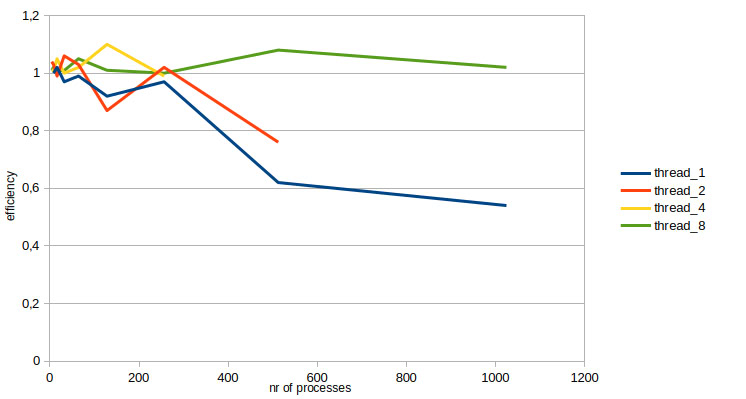
\includegraphics[scale=0.3]{img/efficiency.jpg}
  \centering
  \caption{efficiency graphic}
\end{figure}

\end{multicols}

\bibliographystyle{unsrt}
\bibliography{references}


\end{document}
